\documentclass[letterpaper,twocolumn]{article}
\usepackage[raggedright]{titlesec}
\usepackage[hyphens]{url}
\usepackage{enumerate}
\usepackage{graphicx}
\usepackage{multirow, enumitem, subfigure}
\usepackage[usenames,dvipsnames]{xcolor}
\usepackage{amsmath}
\usepackage{mathtools}
\usepackage{tikz}
\usepackage[normalem]{ulem}
\usepackage{caption}
\usepackage{soul, textcomp}
\usepackage[ruled,vlined]{algorithm2e}
\usepackage{float, comment}
\usepackage{setspace}

\usepackage{lipsum}
\let\OLDthebibliography\thebibliography
\renewcommand\thebibliography[1]{
  \OLDthebibliography{#1}
  \setlength{\parskip}{0pt}
  \setlength{\itemsep}{0pt plus 0.3ex}
}

\newcommand{\rulesep}{\unskip\ \vrule\ }
\newcommand{\soll}{\texttt{Metamorphic and Analytical Guessing of Internet Communications}}
\newcommand{\sol}{\texttt{MAGIC}}

\def\checkmark{\tikz\fill[scale=0.4](0,.35) -- (.25,0) -- (1,.7) -- (.25,.15) -- cycle;} 
\newcommand{\cm}{\checkmark}
%\pagestyle{empty}

\setlength{\textwidth}{7.0in}
\setlength{\textheight}{9.125in}
\setlength{\columnsep}{0.375in}
\setlength{\topmargin}{-0.8in}
\setlength{\oddsidemargin}{-0.25in}
\setlength{\evensidemargin}{-0.25in}
\setlength{\parindent}{0.125in}
\setlength{\parskip}{1mm}

\renewcommand\labelenumi{(\theenumi)}

\date{}

\titlespacing{\section}{0pt}{*2.0}{*2.0}
\titlespacing{\subsection}{0pt}{*1.8}{*1.8}

\renewcommand{\topfraction}{0.9}
\renewcommand{\textfraction}{0.1}

\hyphenpenalty=5000
\tolerance=1000

\begin{document}

\title{\textbf{Systematic Analysis of Network Traffic using MAGIC}}


\author{{\large Utkarsh Goel~\textit{(Student)}, Clint Cooper~\textit{(Student)}, Brittany T. Fasy, and Mike P. Wittie}\\
Department of Computer Science, Montana State University, Bozeman, MT\\
\{utkarsh.goel, clint.cooper, brittany, mwittie\}@cs.montana.edu\\
}
\maketitle 



% Look into Markov Chian creation and see if the results look better. 



\thispagestyle{empty}

\begin{center}
\large\textbf{Abstract}
\end{center}
\vspace{-5pt}

Despite several years of research towards improving user experience with the Web, users remain dissatisfied.
Although, Content Providers make contracts with Content Delivery Networks~(CDNs) and Online Advertisement providers~(OAPs) to speed up webpage load times and improve relevancy of content being shown the website, respectively; however both CDNs and OAPs remain unaware as to what users might be interested in requesting next on the Web.
Therefore, CDNs often fail to prefetch data which prevents further reductions in webpage load times, and OAPs display advertisements based on stale an incomplete Web browsing histories collected for a given user.
In this paper, we present \soll\ (\sol), a technique to passively analyse Web browsing histories and accurately predict users' next interests on the Web.
During our application of \sol\ on real world data, we identified several popular sequences which many users tend to request different websites in.
Based on our observations, we suggest CDNs and OAPs that predicting users' next interests may enable them to collectively further improve the Web experience for the user.
\looseness -1

\medskip
\noindent
\textbf{keywords:} 
Web, behavior, prediction, DNS, MAGIC

\vspace{-8pt}
\section{Introduction}
\vspace{-8pt}
%%%SP

Content providers~(CPs) such as Google, Facebook, Amazon care about high quality of user experience on their websites.
CPs desire that their users remain engaged with their websites, as long user engagement times result in higher number of purchases on the wesbite~\cite{oreilly:businessloss}.
Two of the most important factors that influence user engagement with a website are: 1)~the responsiveness of the website, that is, how fast the website loads after the user clicks a link; and 2)~Whether the website provides content that the user is interested in at the time website is loaded.
As such, CPs employ several sophisticated techniques to speed up the webpage load times and offer the content the user is interested in~\cite{sdch,tcp_fast_open}.
Despite several years of research to improve user experience with the Web, users remain dissatisfied with current Web performance~\cite{rutgers:study}.
We consider the lack of knowledge about users' Web browsing behaviors as the major challenge for CPs to improve user experience.
\looseness -1


%%%TP
\textbf{Content Delivery Networks~(CDNs)} such as Akamai, Level~3, and Limelight are effective in speeding up webpage load times as they distribute application content to their geographically placed Web servers~\cite{cdn}.
A data distribution technique allows users to download website data from a server in close proximity, as opposed to downloading the data from a geographically far server.
However, current content delivery techniques only allow for the content to be distributed to a server proximal to the user's location \textit{only after} the user requests the webpage.
As such, when the requested content is not available from a nearby Web server's cache, the responses take longer as the content needs to be fetched from another CDN server or from a potentially distant CP server.
Consequently, CDNs strive to further reducing webpage loads. They lack the knowledge of users' next Web browsing interests, which can prevent CDN servers from prefetching Web content not available in their cache.
\looseness -1

\textbf{Online Advertisement Providers~(OAPs)} such as Google Ads, Amazon Advertising, and Yahoo! Gemini allow CPs to improve content relevancy on websites according to users' interests.
OAPs are effective in ensuring that advertisements are shown on websites according to recent Web browsing history. 
However, OAPs face two challenges towards ensuring that Web browsing histories are up-to-date and complete.
Firstly, users care about their privacy and thus tend to install browser-based plugins that prevent OAPs to track Web activities of the user.
Secondly, when the user exits the website on which OAPs JavaScript is running, OAPs can not keep track of what next websites the users visit.
Although it is possible for OAPs to host Web proxies and pass all of the user's web requests via that proxy and consequently record user's Web activity, users often show reluctance to use Web proxies.
Therefore, OAPs often remain with an undesired choice of displaying advertisements based on stale or incomplete Web browsing histories of the users.
As such, the displayed advertisements may be irrelevant to user's interests at the time the website is loaded, resulting is degraded user engagement.
\looseness -1




%%%TS
We argue that one of the major challenges to improve user engagement today is the lack of knowledge about users' next Web browsing interests.
Specifically, if CDNs could predict users upcoming browsing interests, website data could be prefetched before it is needed by the user, resulting in even lower webpage load times~\cite{msdn:dns-prefetch,ShangPiggy06}.
Further, if OAPs could also predict users' next interests, they could make well-informed decisions as to which content might be better suited for the user than the techniques they currently use make the same decisions.
In this paper, we investigate Web browsing behaviors of different users and develop techniques that allow for approximate predictions of what users may request next.
We classify the five major contributions of our work as follows:
\looseness -1


\noindent
\textbf{Novelty:} In this paper, we offer an \textit{unaccustomed understanding} of Web browsing behaviors from a large university campus network, with the goal of improving user experience with the Web.
Our investigation includes detailed analysis of network traffic generated by a large student population.
Specifically, our work \textit{predicts} Web browsing behaviors of users using passively collected DNS logs from within the university network.
\looseness -1

\noindent
\textbf{Dataset richness:}  We perform a large scale comprehensive analysis of Web browsing behaviors using a dataset comprising of over 228\,million DNS records collected during a 24-hour period in August 2014.
Further, our dataset comprises of Web browsing sessions from about 12,000 unique users resolving a total of about 700,000 unique domain names embedded on different websites, during the 24-hour period.
\looseness -1

\noindent
\textbf{Implementation:} We introduce \soll~(\sol), a technique to perform a thorough search of website relationships using DNS logs.
\sol~identifies websites that are requested more often in a particular order, thus allowing CDNs and OAPs to accurately predict users' next browsing interests based on which website they have previously visited.
\sol~is effective even when the user leaves a website or installs a browser plugin to prevent websites from tracking browsing history.
In coming days, we plan to make \sol~available to the community as an online tool to calculate popularity of a given list of website names, using the DNS logs collected from a large university campus network.
\looseness -1

\noindent
\textbf{Results:} Based on our experiences with \sol\, we considers our results to be threefold:
\looseness -1

\vspace{-9pt}
\begin{itemize}
    \item We identified several popular sequences of websites that people tend to open in their Web browsers.
    For example, we observed that \textit{Google.com} and \textit{Facebook.com} were the most popular websites that people often visit after visiting any arbitrary website.
    \looseness -1
\vspace{-6pt}
    \item We also observe that for a given sequence of websites, the popularity of the sequence depends on the order in which the websites are requested.
    For example, our data indicates that the popularity of a Web browsing sequence, \textit{Google.com} to \textit{Apple.com} to \textit{Facebook.com}, is significantly different from the popularity of the sequence \textit{Facebook.com} to \textit{Apple.com} to \textit{Google.com}.
    \looseness -1
\vspace{-6pt}
    \item Finally, we observe that when starting the Web browsing session with Google.com, people tend to request a diverse set of websites, than starting the Web browsing for any arbitrary websites -- making the prediction of user's next interest more challenging.
    \looseness -1
\end{itemize}

\vspace{-10pt}

\noindent
\textbf{Inferences drawn:} Based on our results, we make recommendations for CDNs and OAPs that enable them to more effectively serve their purposes for their customers.
Specifically, we suggest CDNs to consider investigating Web browsing behaviors of their users to prefetch any content that may not be available in the cache at the time it is requested.
Finally, we suggest OAPs to predict user's interests to deliver more relevant advertisements on the websites.
\looseness -1

The rest of the paper is organized as follows.
In the next Section~\ref{sec:methodology}, we discuss our approach to collect large scale Web browsing data from a university campus network.
In Section~\ref{sec:technique}, we offer a discussion on our technique to analyse the Web access patterns and predict user's interests on the Web, followed by results in Section~\ref{sec:results}.
In Section~\ref{sec:related_work}, we discuss related work that investigates Web browsing behaviors.
Finally, we conclude in Section~\ref{sec:conclusion}
\looseness -1



 
 

\vspace{-8pt}
\section{Data Collection Methodology}
\label{sec:methodology}
\vspace{-8pt}

Our goal is to discover sequences in which users access different websites. 
To accomplish this goal, we require a metric to uniquely identify users, a chronological list of websites that each user visits, as well as the timestamps of when the websites are visited. 
Therefore, we first discuss the sequence of Internet communication that takes place when a user enters a website URL in the Web browser.
As shown in Figure~\ref{fig:dns_web_req}, in Step~1, the user's Web browser sends a Domain Name System~(DNS) request to a DNS server to resolve the website name into an IP address.
The DNS server replies the user with an IP address~(Step~2).
Next, the user's Web browser creates a connection with the server hosting the IP address returned in Step~2 and sends an Hypertext Transfer Protocol~(HTTP) request to download the website content~(Step~3).
Finally, in Step~4, the Web server sends the website content to user's browser.

In our technique, we choose to collect DNS logs using TCPDump on Montana State University's (MSU) centralized DNS server for a period of 24 hours~\cite{dns:rfc}.
Our inclination to use DNS logs, as opposed to using HTTP logs collected by Web servers~\cite{http:rfc}, is based on the fact that DNS offers a broader view of web browsing behaviors than the HTTP requests alone.
Specifically, several websites use encrypted connections with users' Web browsers.
Therefore, any encrypted HTTP request that the user makes cannot be recorded by monitoring the network, because the content of such HTTP requests is not in plain text and instead is encrypted using public keys.
Whereas the DNS logs are recorded in plain text and contains all website names that the user requests regardless of whether the actual content on the website is download over encrypted or unencrypted connection.
While it is possible to configure Web proxies and monitor user's Web browsing behaviors, users often show reluctance to use Web proxies as such proxies could be malicious and interfere with user's personal information.
In contrast, DNS logs are easily accessible because every user connected to the network would likely use network's default DNS server for resolving domain names.
Therefore, in this study we collected DNS logs from a centralized DNS server hosted by a university campus network.
\looseness -1

  \begin{figure}[t]
\centering
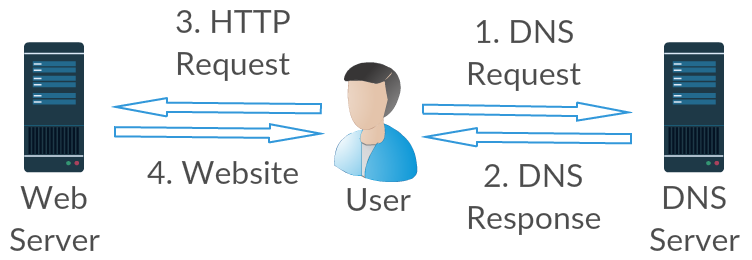
\includegraphics[width=0.8\linewidth]{img/dns_web_req}
\vspace{-5pt}
\caption{Sequence of DNS and HTTP requests being made when visiting a website.}
 \label{fig:dns_web_req}
  \vspace{-19pt}
 \end{figure}

Our collected DNS logs consist of 1)~Users’ IP addresses, which we use to uniquely identify each user; 2)~DNS requests containing domain names of websites visited by the users; and 3)~Epoch timestamps of when DNS requests were sent.
Our current captured DNS logs consists of PCAP files totally about 16\,GB in size.
The PCAP files contains over 228 million DNS records generated during our data collection period.\footnote{A PCAP~(packet capture) file is a binary file that contains information about network requests and traffic.\looseness -1}
\looseness -1

In order to process DNS logs, we first convert the PCAP files to Comma Separated Value~(CSV) files, followed by converting CSV rows to SQL compatible insert statements. 
The process allows us to utilize the well-standardized features of SQL relations to analyze and obtain information from the model.
After correctly storing DNS data into a database, we next sanitize our data and eliminate unwanted DNS data.
Our immediate goal here is to isolate the influence of undesired data from our analysis.
Specifically, we delete DNS responses from the recorded data, this results in the data only containing DNS requests.
We argue that we only need to consider DNS requests, as opposed to both DNS requests and responses, because every DNS requests contains the domain name of the website that the user requests.
Next, we deleted DNS requests which were not destined for our university's centralized DNS server.
Our goal here is to investigate Web browsing behavior for users that use university's DNS server for requesting all the websites.
Finally, we delete DNS requests that seek IPv6 IP addresses.
We argue that we only require DNS requests that resolve to an IPv4 address, because Web browsing behaviors are irrespective of which IP protocol version users' networks supports.
Our sanitized data consists of over 12 million DNS requests for about 12000 unique IP addresses accessing over 700,000 domains in a 24-hour period.
\looseness -1



\vspace{-10pt}
\section{Implementation Details}
\label{sec:technique}
\vspace{-8pt}

To analyze the DNS data and identify popular sequences of websites that users often visit, we developed \sol.
As shown in Algorithm~1, \sol\ allows generation of HashMaps, where a HashMap is a key-value pair of a sequence of different domain names with the number of times the sequence is requested.
\looseness -1

\begin{figure}[t]
\centering 
 \minipage{0.49\textwidth}
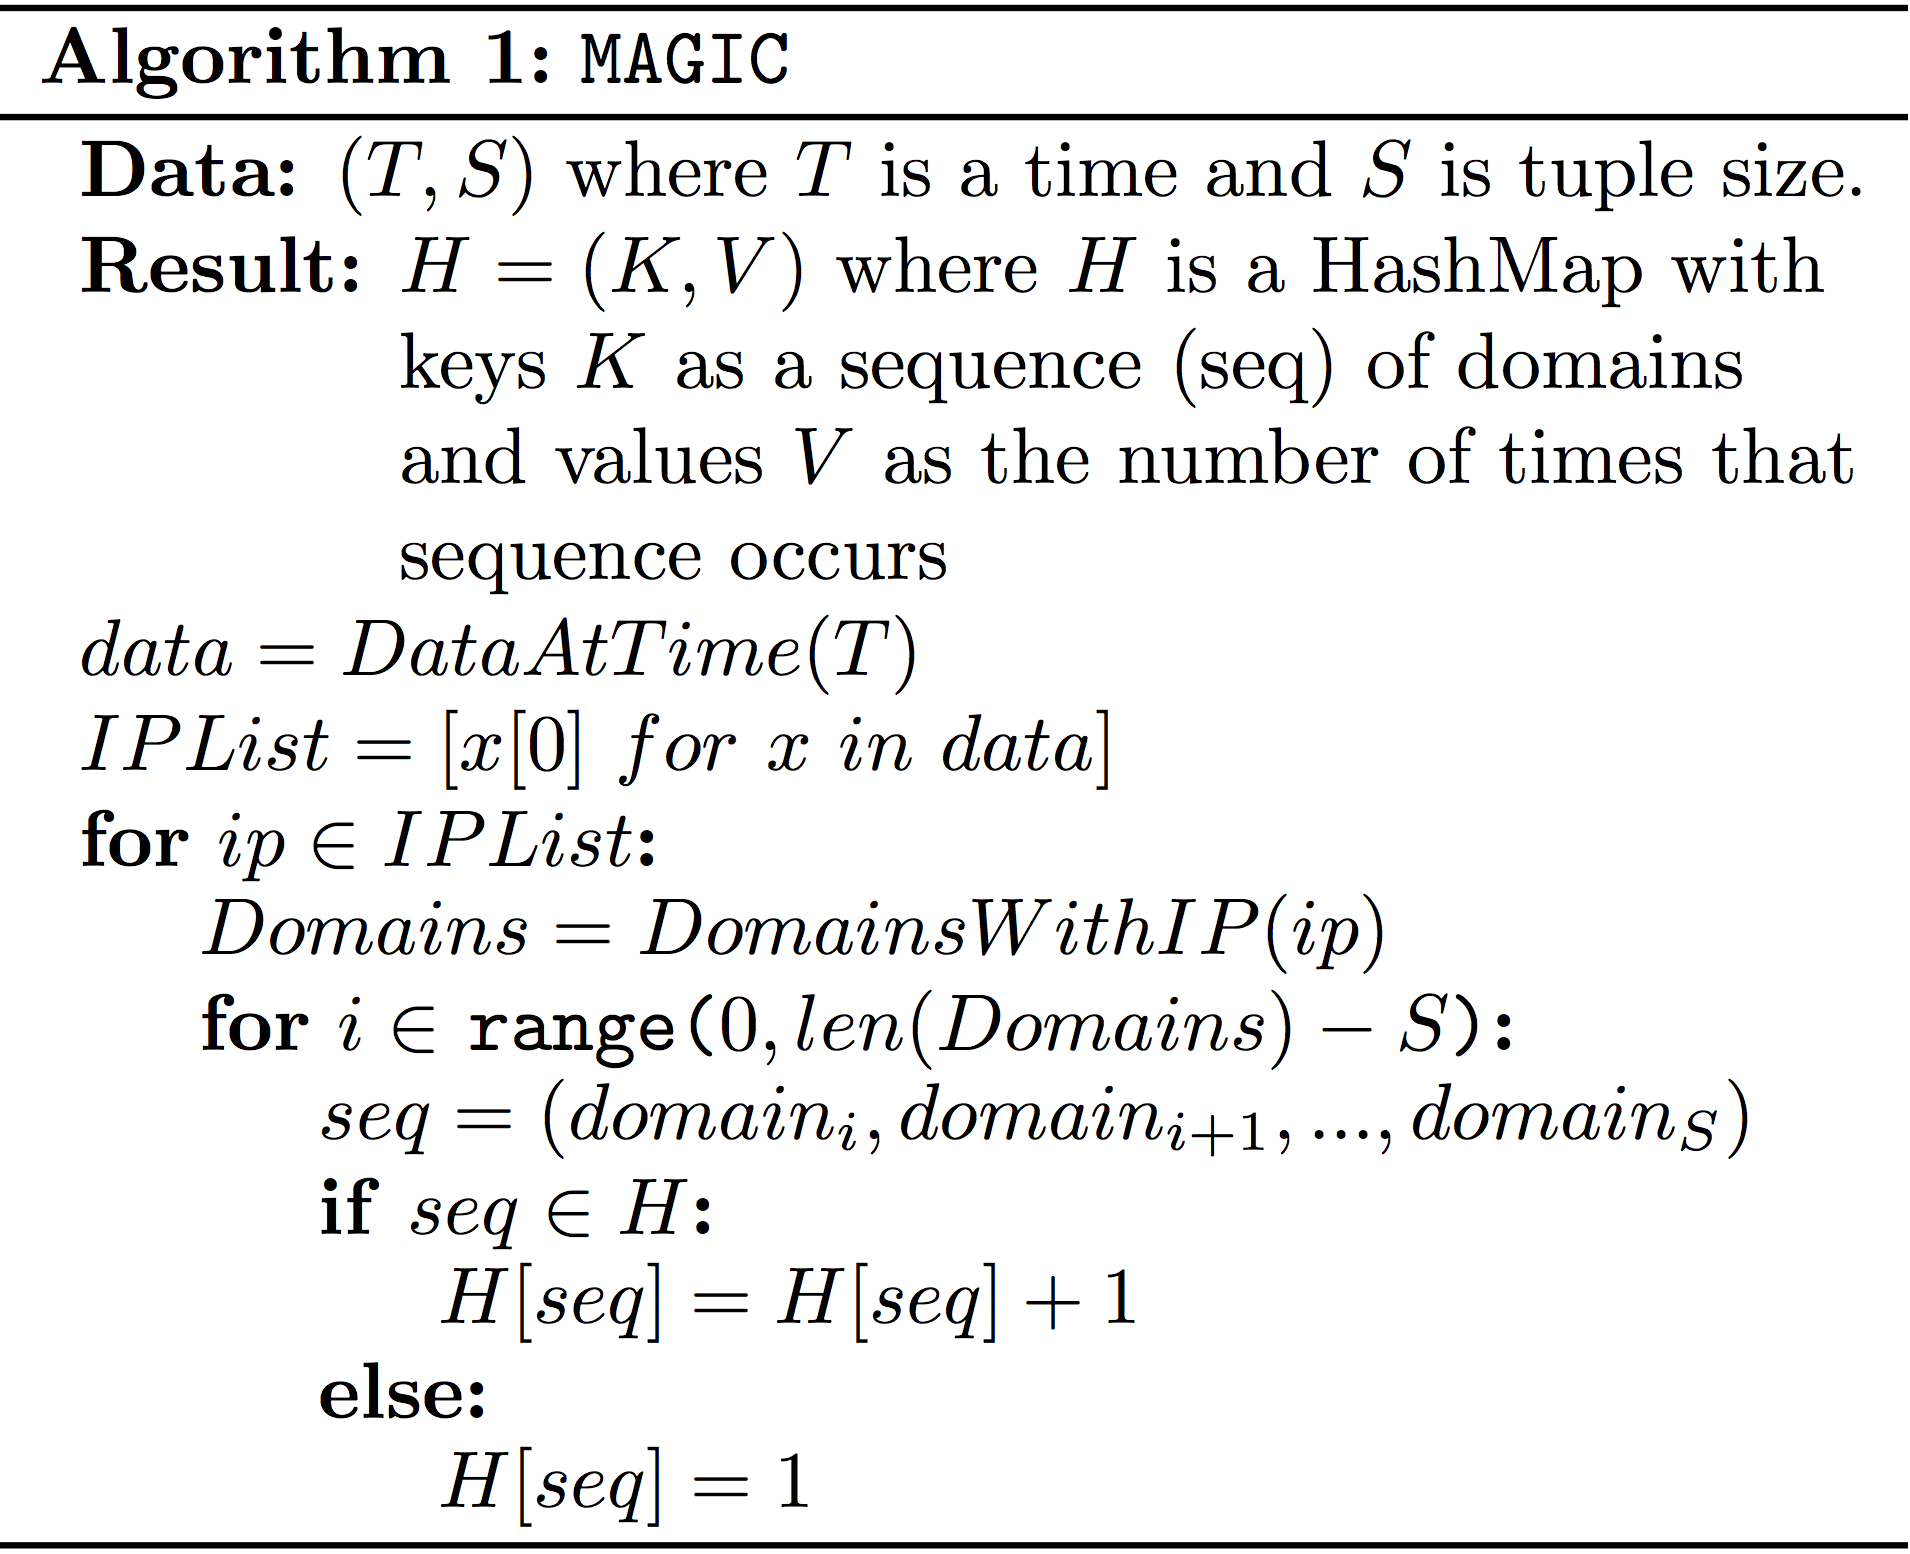
\includegraphics[width=\linewidth]{img/magic}
  \vspace{-28pt}
   \endminipage
\end{figure}



\begin{figure*}[t]
\centering 
 \minipage{0.49\textwidth}
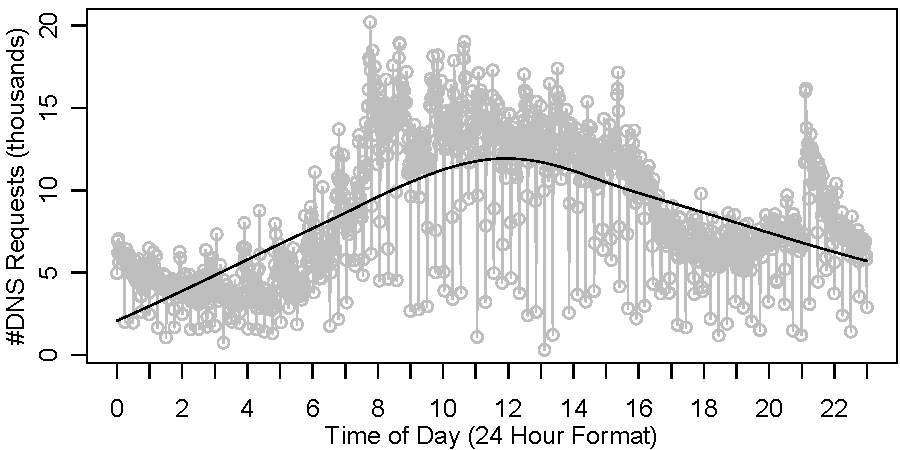
\includegraphics[width=\linewidth]{img/total_dns_over_time}
  \vspace{-15pt}
\caption{Distribution of the total number of DNS requests over a period of 24 hours.}
 \label{fig:total_dns_hit}
  \endminipage
  \hfill
  \minipage{0.49\textwidth}
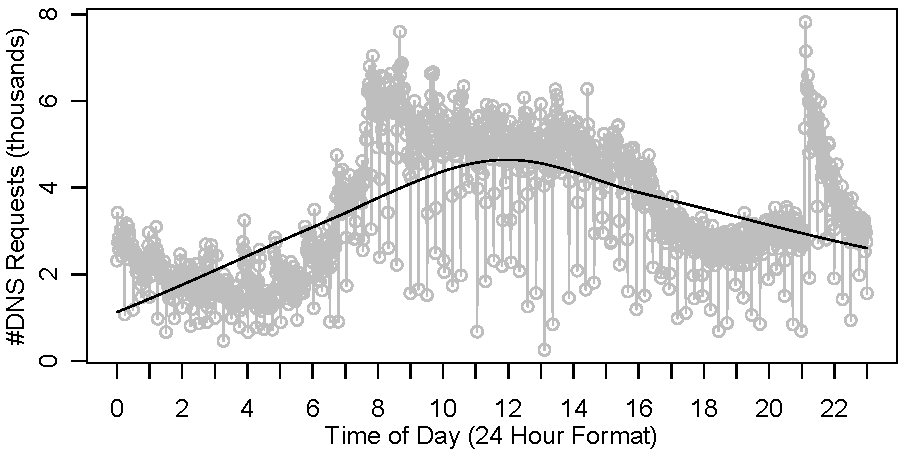
\includegraphics[width=\linewidth]{img/unique_dns_over_time}
  \vspace{-15pt}
\caption{Distribution of the number of unique DNS requests over a period of 24 hours.}
 \label{fig:unique_dns_hit}
  \endminipage
  \vspace{-10pt}
 \end{figure*}
 
    \begin{figure*}[t]
\centering
 \minipage{0.49\textwidth}
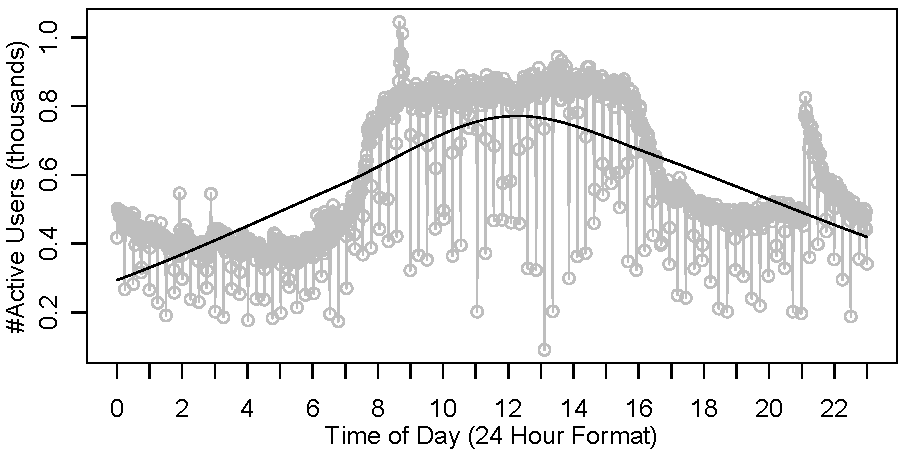
\includegraphics[width=\linewidth]{img/active_users_over_time}
  \vspace{-15pt}
\caption{Distribution of the unique number of active users over a period of 24 hours.}
 \label{fig:active_users}
  \endminipage
  \hfill
  \minipage{0.48\textwidth}
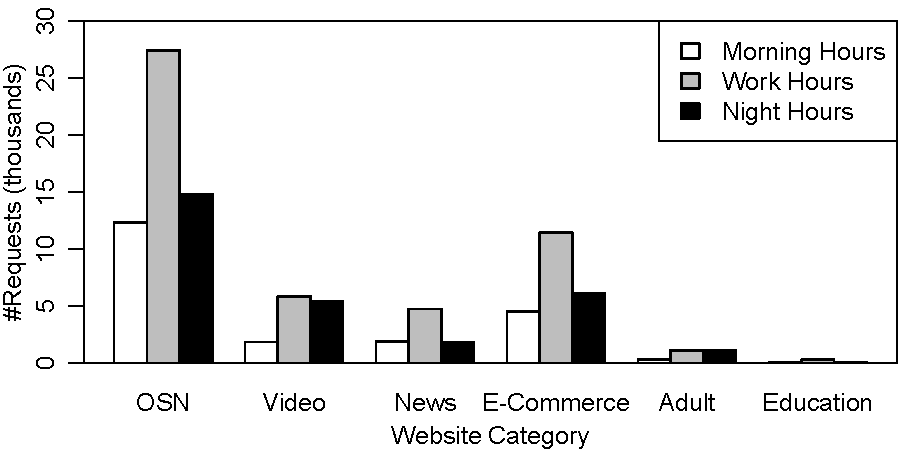
\includegraphics[width=\linewidth]{img/popularity}
  \vspace{-15pt}
\caption{Popularity of websites classified under various categories of online services.}
 \label{fig:popularity_per_hour}
  \endminipage
  \vspace{-18pt}
 \end{figure*}

We design \sol\ to accept user defined arguments, such as the time of day $T$ and a desired sequence size $S$.
Next, \sol\ generates a list of sequences and sequence request counts.
As shown in Algorithm~1, we use SQL queries $DataAtTime$ and $DomainsWithIP$ to obtain IP addresses and domain names associated with each IP address, respectively. 
For every IP address extracted with $DataAtTime$ query, we fetch domain names in chronological order and generate sequences of website visits that are of length $S$. 
These sequences represent keys in the HashMap $H$.
The associated count value is initialized as 1 and incremented for each occurrence of the same sequence.
The resulting HashMap is returned to the user once all IP addresses within $IPList$ are processed and added as sequences to the HashMap.
\looseness -1



 


\vspace{-8pt}
\section{Putting \sol\ in Context}
\label{sec:results}
\vspace{-8pt}

We now employ \sol\ to investigate and understand Web browsing behaviors using our collected DNS data.
However, our first goal is to understand whether or not our data constitutes a substantial number of DNS records at any point in time, allowing us to reliably predict Web browsing behaviors.
\looseness -1

\vspace{-8pt}
\subsection{Data Significance}
\vspace{-8pt}

In Figure~\ref{fig:total_dns_hit}, we show the total number of sanitized DNS requests that the university's DNS servers received over a period of 24 hours.
The x-axis represents time duration in a 24-hour format.
The y-axis represents the number of DNS requests received by the DNS server.
The greyed scatter plot represents actual number of DNS requests, whereas the solid line, represents the regression for the distribution. 
From the figure we see that at any given point in time during the day, our dataset consists of over 5000 DNS requests.
Moreover, when analysing DNS requests for unique domain names in Figure~\ref{fig:unique_dns_hit}, we observe that our dataset consists of at least 3000 DNS requests at any given point in time.
\looseness -1

Finally, we investigate whether our dataset consists of DNS requests from substantial number of unique users at any given time of the day.
In Figure~\ref{fig:active_users}, we show the distribution of active users at different times of a day.
Similarly to previous figures, the x-axis represents time of day in a 24-hour format.
The y-axis represents the total number of active users or unique IP addresses in our dataset.
From the figure we observe that at any given time of a day our dataset consists of DNS requests generated by 500 unique users on average. 
Similarly to Figure~\ref{fig:total_dns_hit}, we observe that during the peak hours~(8AM to 5PM) the number of active users are also at a maximum.
Therefore, based on the data we collected, we argue that such a large dataset is statistically significant to allow us to make reliable observations about Web browsing behaviors of different users.
\looseness -1


 \begin{figure*}[t]
\centering
\minipage{0.49\textwidth}
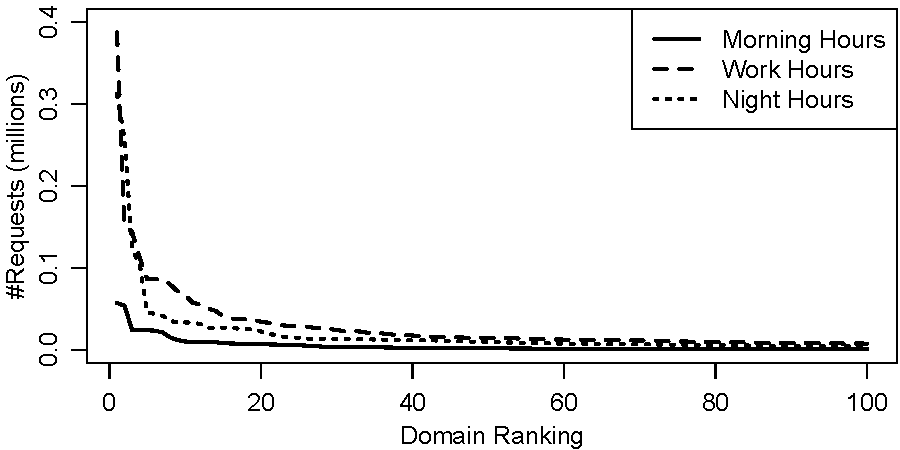
\includegraphics[width=\linewidth]{img/domain_popularity_over_time}
\vspace{-17pt}
\caption{Distribution of visits to top 100 websites.}
 \label{fig:domain_popularity}
  \endminipage
  \hfill
  \minipage{0.49\textwidth}
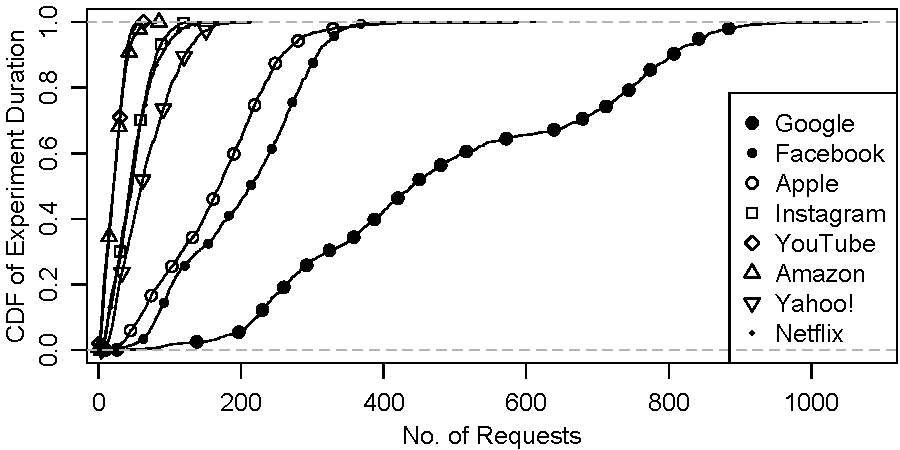
\includegraphics[width=\linewidth]{img/website_popularity_cdf}
\vspace{-17pt}
\caption{Distribution of visits to top 8 websites.}
 \label{fig:website_popularity_per_hour}
  \endminipage
  \vspace{-15pt}
 \end{figure*}


\vspace{-8pt}
\subsection{Data Classification}
\vspace{-8pt}

Next, we are interested in understanding the popularity of different types of online services across different times of a day.
Our goal here is to understand whether or not some online services are visited more often than others.
In Figure~\ref{fig:popularity_per_hour}, we show that different online services tend to exhibit different popularities, especially at different times of a day.
The x-axis on the figure represents six different popular online service groups.
The y-axis represents the popularity of each service, where we define popularity as the number of DNS requests served by the DNS server.
The white, gray, and black bar graphs represent the popularity in morning~(5\,AM to 8\,AM), work~(8\,AM to 5\,PM), and night(5\,PM to 5\,AM) hours respectively.
\looseness -1

\begin{table}[t]
\centering

\begin{tabular}{l|l}
\textbf{Category} & \textbf{Websites}                                                                                     \\ \hline \hline
OSN               & \begin{tabular}[c]{@{}l@{}}G+, FaceBook, Twitter,  LinkedIn\end{tabular}                   \\ \hline
Video             & \begin{tabular}[c]{@{}l@{}}YouTube, Netflix, Hulu, Vimeo, \\ DailyMotion, HBO\end{tabular}            \\ \hline
News              & \begin{tabular}[c]{@{}l@{}}CNN, Fox, HuffingtonPost, Reddit, \\ NYTimes, Yahoo News\end{tabular}      \\ \hline
E-Commerce        & \begin{tabular}[c]{@{}l@{}}Walmart, Target, Ebay, BestBuy, \\ Amazon, Costco, Craigslist\end{tabular} \\ \hline
Adult             & Top adult websites~\cite{topporn}                                                              \\ \hline
Education               & D2L, ECats                                                                                            \\ \hline
\end{tabular}
\vspace{-5pt}
\caption{List of websites classified under different categories based on the service they offer.}
\label{tbl:domain_classify}
\vspace{-21pt}
\end{table}

From the figure, we see that the number of websites visited by people in the morning and evening are about one-third of the number of websites visited during the work hours.
For example, Online Social Networks~(OSN) such as Facebook, LinkedIn, Google Plus, or Twitter, are visited almost twice as much during the work hours as they are during the morning and night hours.
Similarly to OSN websites, online services that offer e-commerce and news tend to be visited more during work hours.
However, video streaming and porn websites show similar popularity during both the work and night hours.
Surprisingly, although the Desire-2-Learn~(D2L) website is used by students and faculty throughout MSU colleges to access study materials, our data indicates that D2L is not visited as much as other online services at any time in the day.
We speculate that such an observation could potentially be an artifact of the day we collected the DNS records, however, for the purpose of this work, we do not plan to investigate such potential artifacts and leave them for future data analysis studies.
For interested readers, in Table~\ref{tbl:domain_classify}, we list the various websites which we selected to classify the online services described in Figure~\ref{fig:popularity_per_hour}.
\looseness -1

 \begin{figure}[t]
\centering
 \minipage{0.49\textwidth}
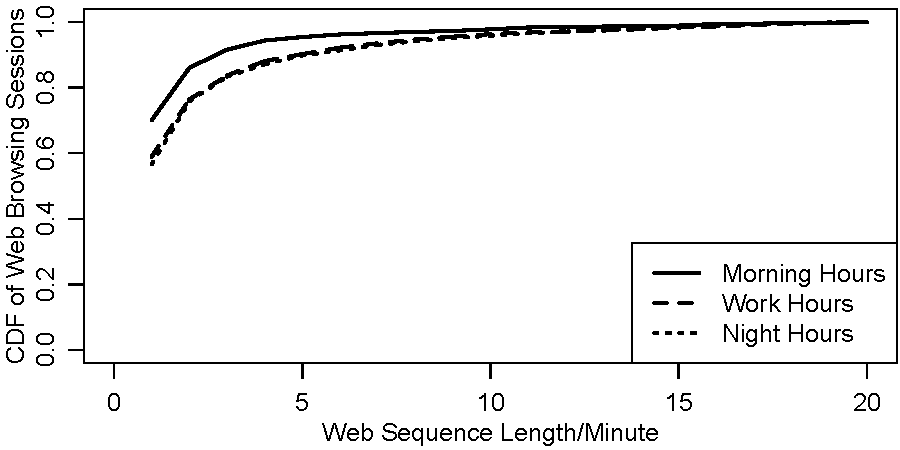
\includegraphics[width=\linewidth]{img/sequence_length}
\vspace{-15pt}
\caption{Distribution of the number of websites visited every minute.}
 \label{fig:sequence_length}
  \endminipage
  \vspace{-23pt}
 \end{figure}

Next, we investigate the popularity of all the websites to understand whether there exist websites that users visit more often than the other websites. 
Additionally, we investigate most popular websites tend to change over time.
In Figure~\ref{fig:domain_popularity}, we show the difference in how many times different websites are requested by users.
The x-axis shows the rank of the top 100 websites, based on how often they were requested.
The y-axis shows the number of times the top 100 websites are requested.
The different lines represent the requests at different times of the day.
As we observe from the figure, users tend to visit only about 8 websites more often than other websites, regardless of time of the day.
\looseness -1

 
\begin{figure*}[t]
\centering
\minipage{0.75\textwidth}
\vspace{-35pt}
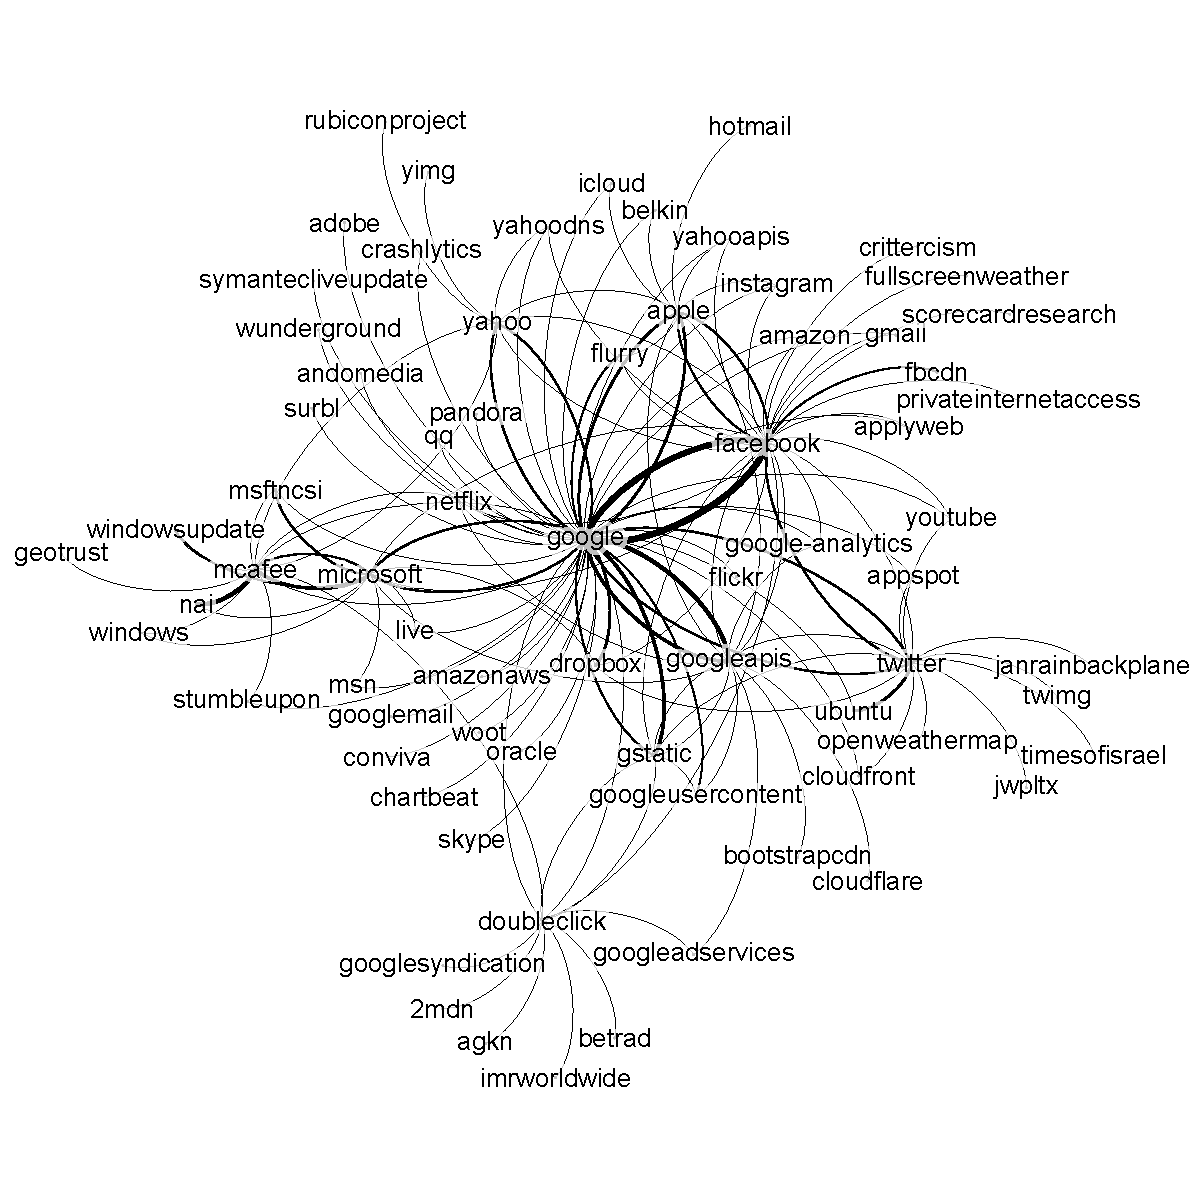
\includegraphics[width=\linewidth]{img/MorningLength2Cluster}
\vspace{-50pt}
\caption{Popularity of different websites in the morning hours.}
 \label{fig:morning}
\endminipage
    \vspace{-15pt}
 \end{figure*}


\begin{figure*}[t]
\centering
 \minipage{0.87\textwidth}
 \vspace{-75pt}
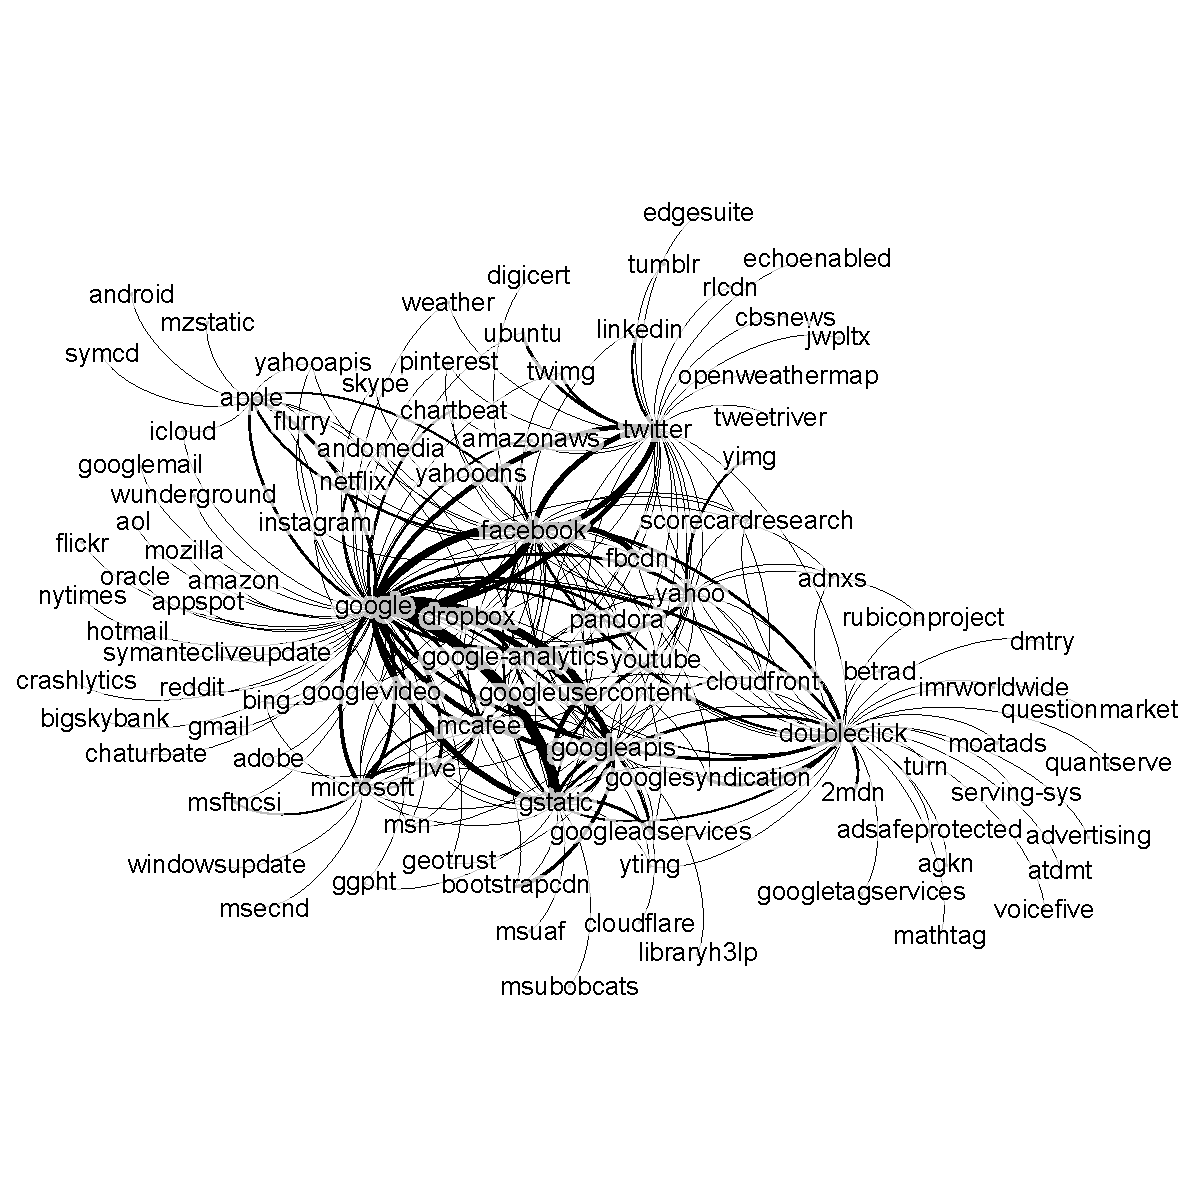
\includegraphics[width=\textwidth]{img/WorkingLength2Cluster}
\vspace{-88pt}
\caption{Popularity of different websites in the working hours.}
 \label{fig:work}
 \vspace{-15pt}
\endminipage
 \end{figure*}
 
 \begin{figure*}[t]
\centering
 \minipage{0.75\textwidth}
 \vspace{-45pt}
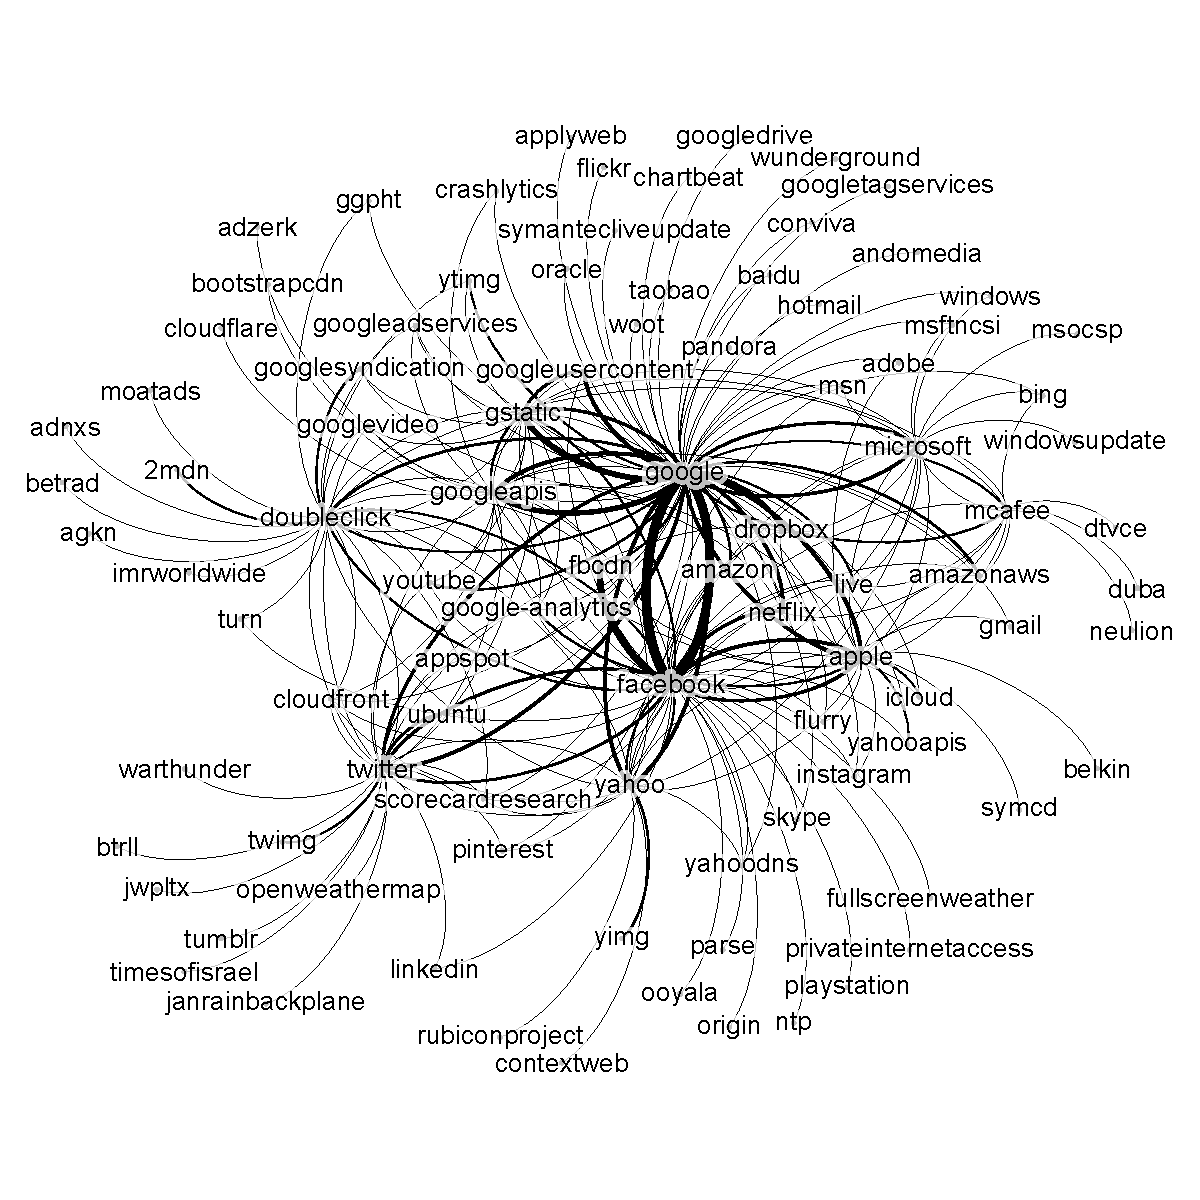
\includegraphics[width=\linewidth]{img/EveningLength2Cluster}
\vspace{-55pt}
\caption{Popularity of different websites in the evening hours.}
 \label{fig:evening}
\endminipage
    \vspace{-15pt}
 \end{figure*}

Therefore, in Figure~\ref{fig:website_popularity_per_hour}, we show the popularity of the top 8 websites in terms of how often users visit these websites throughout the day.
The x-axis in the figure represents number of times a given website is requested.
The y-axis represents a CDF of experiment duration during the day.
From the figure we observe that about 40\% of the time, \textit{Google.com} is requested atleast 500 times every minute.
Whereas, users visit other websites such as \textit{Facebook.com} or \textit{Apple.com} only about 200 times a minute. 
We argue that because some websites are visited less often than other websites, there may exist some scenarios when websites tend to be visited more than in other scenarios.
Specifically, what remains unclear is whether some websites are requested more often after a specific website is opened or the requests for websites are completely random.
Therefore, in the next section we investigate whether users tend to have a sequence in which websites are requested.
 \looseness -1

 
\vspace{-12pt}
\subsection{Identifying Website Sequences}
\vspace{-10pt}

Interactive websites today consists of content that lead users from one website to another website with related content.
While it is possible that users sequentially visit a number websites when looking for specific information online, it would be practically challenging to prefetch the data pertaining to all the websites that the users visit.
Therefore, we first investigate the number of websites users often visit.
Our immediate goal here is to identify the most popular length of sequences of websites that users visit.
In Figure~\ref{fig:sequence_length}, we show a distribution of length of sequences that users visit in order.
The x-axis represents the number of websites users visits every minute.
The y-axis represents a CDF of Web browsing sessions.
We can observe from the figure that about 80\% of the browsing sessions only consists of visits to 2 websites.
Therefore, we argue that investigating popular sequences of only length two would enable us to understand Web browsing behaviors.
\looseness -1

Finally, we use \sol\ to identify popular sequences of website visitation that are of length two.
In Figures~\ref{fig:morning}-\ref{fig:evening}, we show Web browsing behaviors in the morning, working, and evening hours. 
The labels represent websites visited by different users.
The edges represent a causal relationship between the two websites.
Specifically, directionality of edges is represented using a clockwise direction where the direction represents the users' interests from visiting a \textit{Source website} followed by visiting a \textit{Destination website}.
The thickness of an edge represents the frequency of the visitation, that is, how often users visit from one website to another.
\looseness -1

In general, we observe from the figures that most of the Web traffic originates from a few websites such as \textit{Google}, \textit{Facebook}, \textit{Twitter}, Yahoo!, \textit{DoubleClick}.
Moreover, these websites contribute most of the traffic during morning, working, and evening hours. 
For example, the connection between \textit{Facebook} and \textit{Google} persists to be the most popular connection across all three figures. 
Our previous results~(Figures \ref{fig:total_dns_hit}, \ref{fig:unique_dns_hit}, and \ref{fig:active_users}) indicate that the Web traffic during work and evening hours is significantly larger than traffic in the morning hours.
We observe similar trend in Figures~\ref{fig:work} and~\ref{fig:evening}, as we observe larger number of websites being visited by users during these hours.
Finally, we observe that although \textit{YouTube} is popular online video streaming service, we do not observe a lot of Web traffic to or from YouTube.
We speculate that users tend to visit \textit{YouTube} directly, as opposed to visiting it after other website, and stay long enough that it becomes unlikely to predict user's next Web browsing interests. 



\begin{comment}
\begin{figure*}[]
\centering
 \minipage{0.99\textwidth}
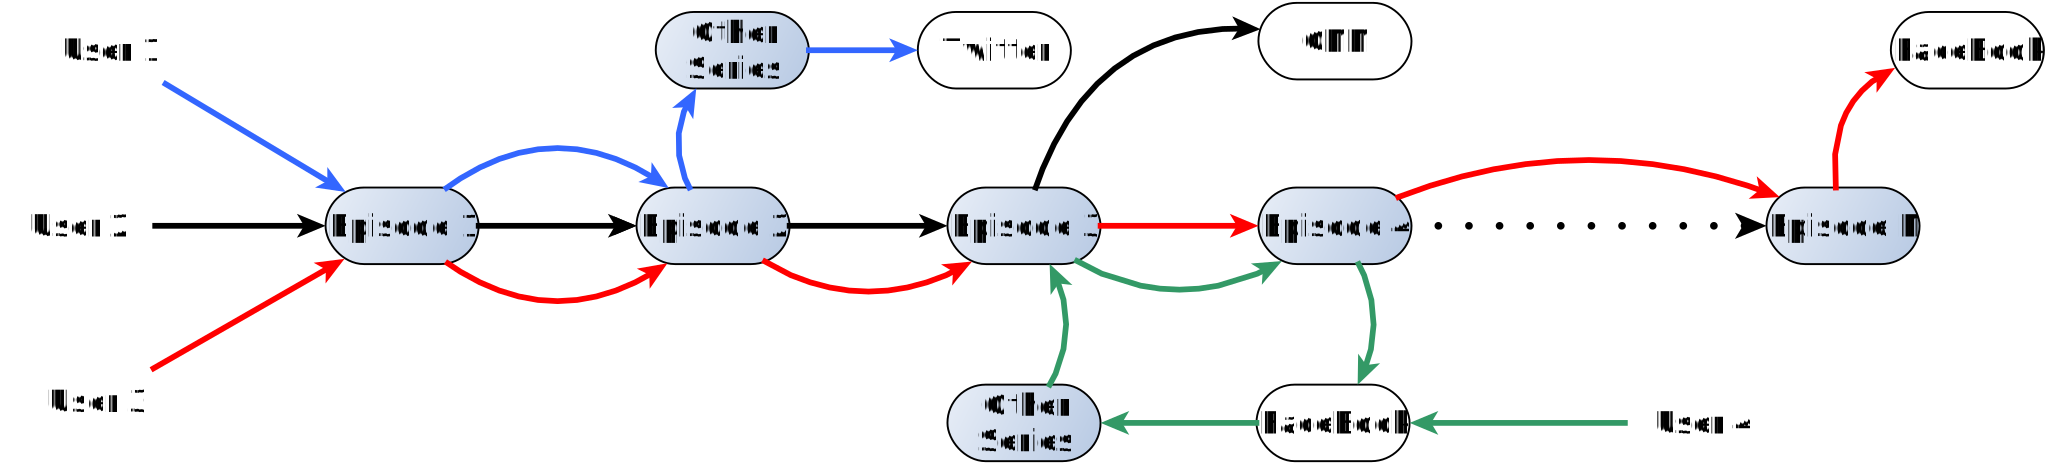
\includegraphics[width=\linewidth]{img/WatchPattern}
\caption{A contrived topology of how different users may browse the Web.}
 \label{fig:watch_pattern}
  \endminipage
  \vspace{-10pt}
 \end{figure*}



\vspace{-8pt}
\section{Discussion}
\label{sec:discussion}
\vspace{-8pt}

We believe predicting Web browsing interests of different users can enable CDNs to proactively predict user’s subsequent requests and make the needed data available in the cache before the user requests it. 
For example, when content for website A is not be available in CDN's cache at the time it is requested, CDNs fetch the requested content from origin servers, which increases time to load web pages because origin servers are often very far from CDN servers.
However, if prediction on Web browsing behaviors indicate that users often visit website \textit{B} after visiting website \textit{A}, CDNs could proactively fetch content related to website \textit{B} from origin servers while the user is loading content for website \textit{A}.
\looseness -1

We also believe that our technique would inspire advertisers to improve the advertisements they currently display on websites.
Currently, advertisers present advertisements based on the websites that users have already visited. 
For example, a major online advertiser in the US provides advertisements for similar content to what a user searches for on the website.
However, if a user has already purchased the product, the corresponding advertisement may not be relevant to the user. 
Based on our results, we argue that online advertisers could perform a prediction as to what the user might be interested in next and consequently customize advertisements according to user's upcoming interests. 
\looseness -1

\end{comment}






\vspace{-15pt}
\section{Related Work}
\label{sec:related_work}
\vspace{-8pt}

Several studies investigate popularity, type, and amount of time spent on websites visited by users~\cite{BighamCBWL07,export:176481,Huang:2010:PBB:1810617.1810622,montgomery2000trends}.
Other studies estimate gender, age, and identiy of users by just analysing Web browsing behaviors~\cite{275,canali2014effectiveness,Hu:2007:DPB:1242572.1242594,kakkarweb}.
With respect to implementation, several studies develop and investigate algorithms to predict Web browsing behaviors~\cite{awad2012prediction,dongre2015improved,scott2006nested,shiryayev1992markov,zhu2005behavior}.
In contrast to above studies, our work identifies actual sequences of websites visited by using DNS logs, as opposed to user-sensitive HTTP logs.
\looseness -1







\begin{comment}
\vspace{-8pt}
\section{Future Work}
\label{sec:future_work}
\vspace{-8pt}

While inspecting DNS logs allows observing Web browsing behaviors and prefetching content related to users' next Web browsing interests, what remains unclear is when to perform the prefetch.
However, time-sensitive prefetches need to be personalized based on individual user's Web browsing behavior.
For example, as shown in Figure~\ref{fig:watch_pattern}, let us assume that \textit{User~1}, \textit{User~2}, and \textit{User~3} start their Web browsing sessions by requesting \textit{Episode~1} from an online video streaming website. 
\textit{User~1} watches the first two episodes and then decides to watch a different series on the same video streaming website, ultimately ending her video streaming session and requesting \textit{Twitter.com}. 
\textit{User~2} behaves similarly, but requests the homepage of \textit{CNN.com} after watching \textit{Episode~3}. 
\textit{User~3} watches all available episodes of the same series one after another and then requests the homepage of \textit{Facebook.com}. 
\textit{User~4} currently on \textit{Facebook.com}, finds an interesting article about Episode~3, making her want to end her browsing session on \textit{Facebook.com} and stream Episode~3.
\textit{User~4} requests \textit{Episode~4} after watching \textit{Episode~3}, after which she ends her video streaming session to return to \textit{Facebook.com}. 
\looseness -1

For \textit{User~1}, content corresponding to \textit{Twitter.com} needs to be fetched after the user finishes watching two episodes and $n$ number of episodes from the other series. 
$n$ is a known value calculated by examining the sequence of watched episodes across different series. 
For \textit{User~2}, corresponding to \textit{CNN.com} needs to be fetched after user finishes watching three episodes.
However, for \textit{User~3} it remains unclear as to when to prefetch content corresponding to \textit{Facebook.com} as the user spends a long and undetermined amount of time streaming several episodes.
Predictions for this user become trivial as she will most likely continue to watch episodes. 
Finally, for \textit{User~4}, content corresponding to the video streaming website needs to fetched as soon as the user visits \textit{Facebook.com}.
Additionally for the same user, content related to \textit{Facebook.com} needs to be fetched after the user finishes watching episodes 3 and 4 as well as $n$ number of episodes from the other series..
\looseness -1

Based on the above hypothetical example, we argue that inspecting both DNS and HTTP logs together would enable us to identify when the prefetch for users' next Web interests could be performed.
However, we consider such analyses out of the scope of this paper and leave that as the future work.
\looseness -1
\end{comment}







\vspace{-12pt}
\section{Conclusions}
\label{sec:conclusion}
\vspace{-10pt}

Despite several years of research, websites often struggle to deliver an enjoyable experience that the users want to enjoy.
one of the major challenges for Web servers to improve Web experience for users is to make the data available before it is requested by the client, thereby reducing latency to generate and transmitting the response to the client devices.
In this paper, we present \sol\, a technique to passively analyse users' Web browsing histories and suggest their next Web browsing interests with a probability.
During our application of \sol\ on real world data, we identified several popular sequences which many users tend to request different websites in.
We suggest CDNs and OAPs that predicting users' next interests may enable them to collectively further improve the Web experience for the user.
\looseness -1




\vspace{-10pt}
\section*{Acknowledgments}
\vspace{-8pt}
The authors would like to thank Mike Hitch at the IT Center of Montana State University to provide us university-wide DNS logs.
We also thank \mbox{National} \mbox{Science} \mbox{Foundation} for supporting this work through the grant \mbox{NSF CNS-1555591}.
Finally, we thank Montana State University for supporting Clint Cooper through a Presidential scholarship.
\looseness -1


\vspace{-11pt}
\bibliographystyle{plain}
\bibliography{topo} 

\end{document}
